\documentclass[10pt, xcolor=x11names,compress]{beamer}
%\usecolortheme{seagull}
%\usecolortheme{crane}
%\useoutertheme{infolines}
\usefonttheme[onlymath]{serif}
%\setbeamertemplate{headline}[default]
\setbeamertemplate{navigation symbols}{}
\mode<beamer>{\setbeamertemplate{blocks}[rounded][shadow=true]}
\setbeamercovered{transparent}
\setbeamercolor{block body example}{fg=blue, bg=black!20}


%Information to be included in the title page:
\title{vLUME paper + Deep Learning\\... and why you may care}
\author{Anton Popov}
\institute{ViRe / IJC}
\date{14/12/2020}

\useoutertheme[subsection=false]{miniframes}

\begin{document}

\frame{\titlepage}

\section{Introduction}

\subsection{Subsection1}
\begin{frame}
	\begin{figure}
		\centering
		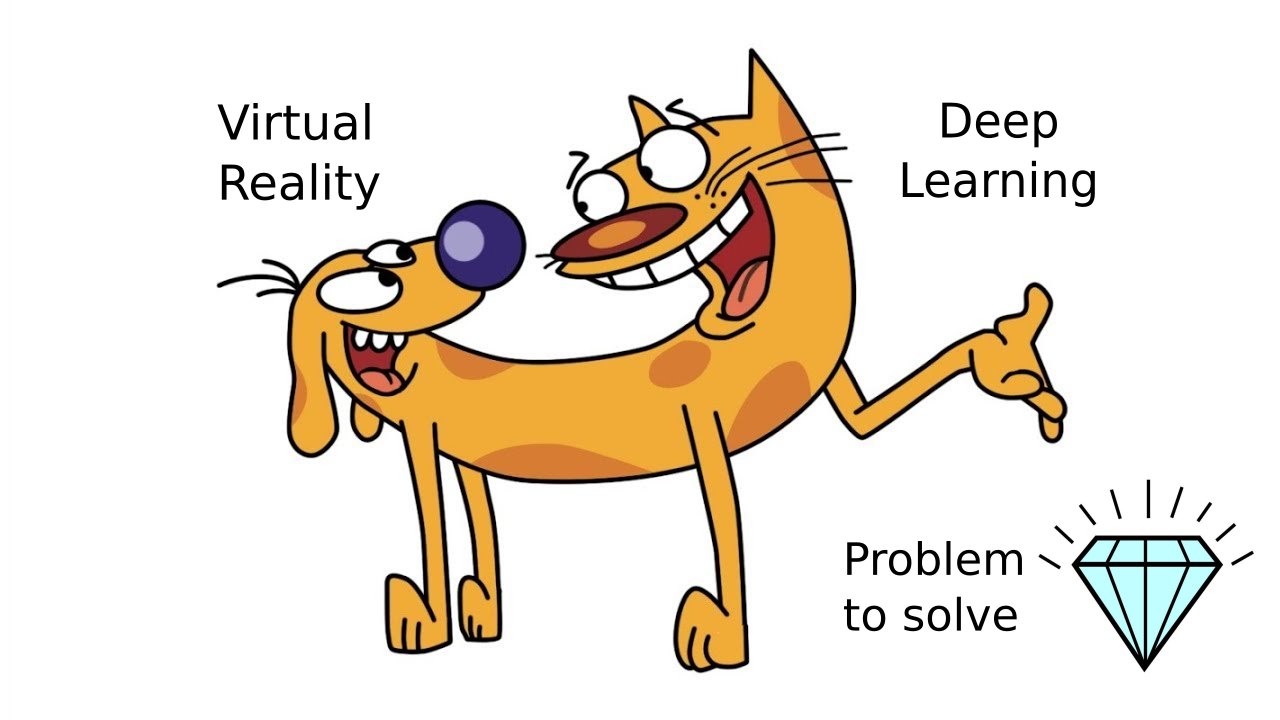
\includegraphics[height=.75\textheight]{images/cat-dog-gem.png}
	\end{figure}
\end{frame}


\section{vLUME paper}

\subsection{Subsection1}
\begin{frame}
	% image with Daniel's name highliting
	\begin{figure}
		\centering
		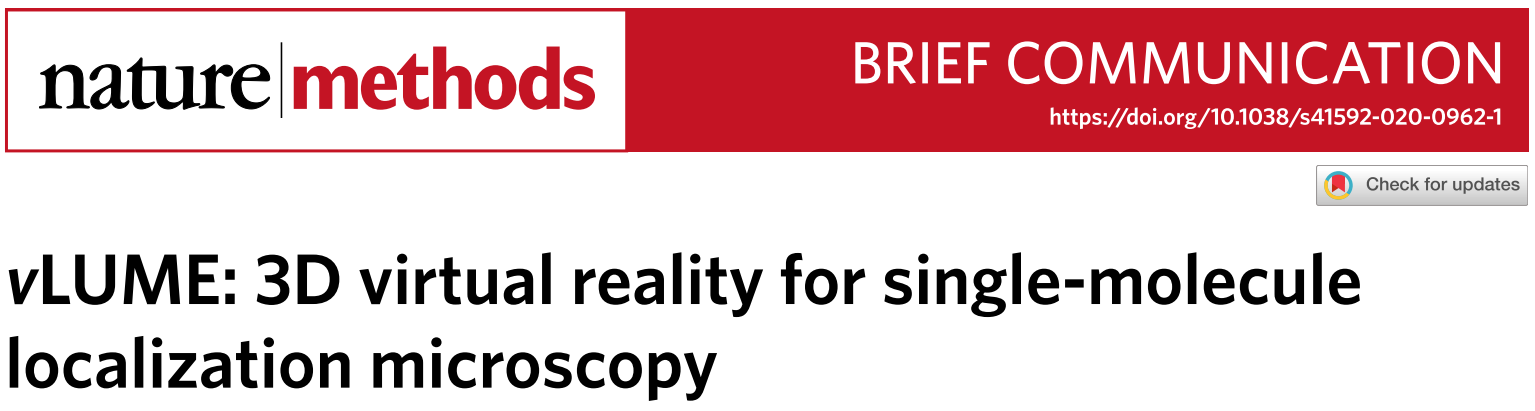
\includegraphics[height=.35\textheight]{images/paper.png}
	\end{figure}
by Daniel Esteban-Ferrer \textit{et al.}
\end{frame}

\subsection{Subsection2}
\begin{frame}
\frametitle{Definition}
	\begin{columns}
	\begin{column}{0.45\textwidth}
		\begin{figure}
			\centering
			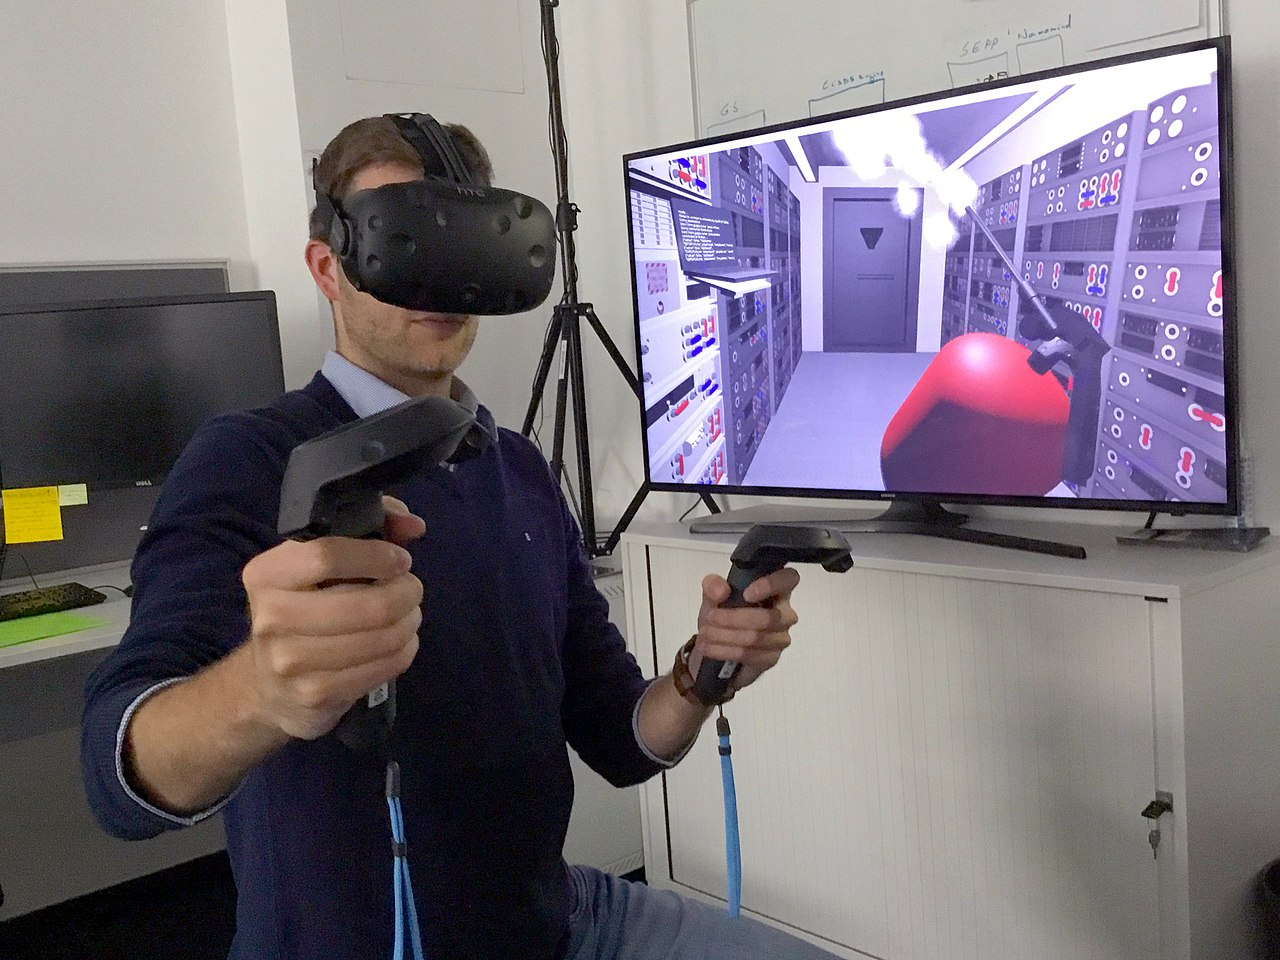
\includegraphics[width=\textwidth]{images/vr.jpg}
		\end{figure}
	\end{column}
	\begin{column}{0.55\textwidth}
		\begin{alertblock}{Virtual reality (VR)}
			the use of computer modeling and simulation that enables a person to interact with an artificial three-dimensional (3-D) visual or other sensory environment.
		\end{alertblock}
		\begin{block}{But why?}
			Human spatial perception is fundamentally 3D.
		\end{block}
	\end{column}
\end{columns}
\end{frame}

\subsection{Subsection3}
\begin{frame}{Demo}
	%https://www.youtube.com/watch?v=6yx_sayhsiA&feature=youtu.be
	\begin{center}
%		\href{run:/snap/bin/vlc  video/demo.mp4}{
		\href{https://www.youtube.com/watch?v=6yx_sayhsiA&feature=youtu.be}{
		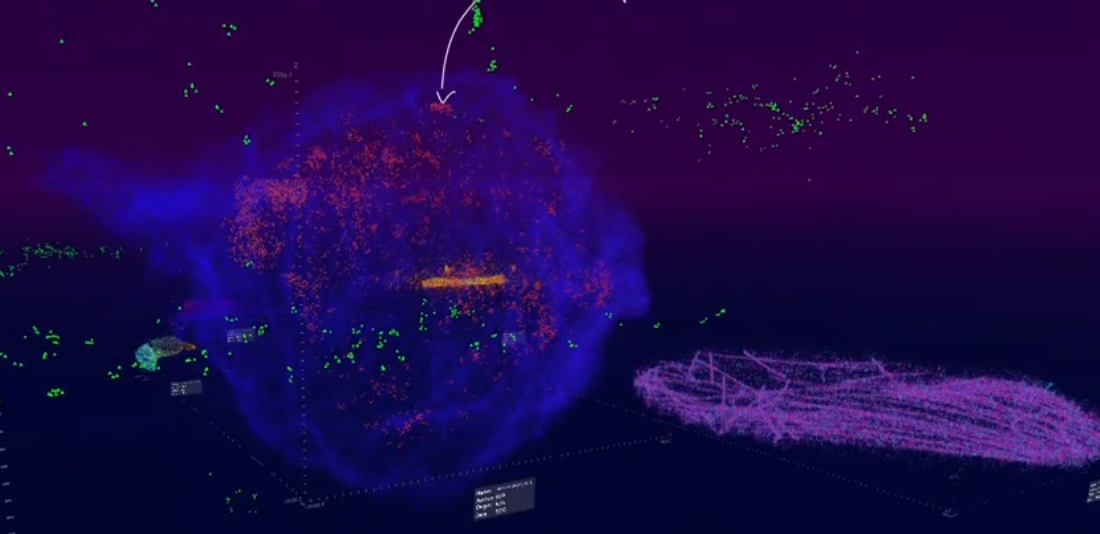
\includegraphics[scale=0.25]
		{images/demo.png}
	}
	\end{center}
\end{frame}

\subsection{Subsection4}
\begin{frame}{vLUME's key features}
	\begin{enumerate}
		\item Data exploration and comparison
		\item 3D regions of interest extraction (ROI); annotation, segmentation
		\item Custom analysis of user-defined subregions
		\item Export of video files for presentations / publications
	\end{enumerate}
\end{frame}


\subsection{Subsection5}
\begin{frame}
	\frametitle{Conclusions}
	\begin{columns}
		\begin{column}{0.4\textwidth}
			\centering
			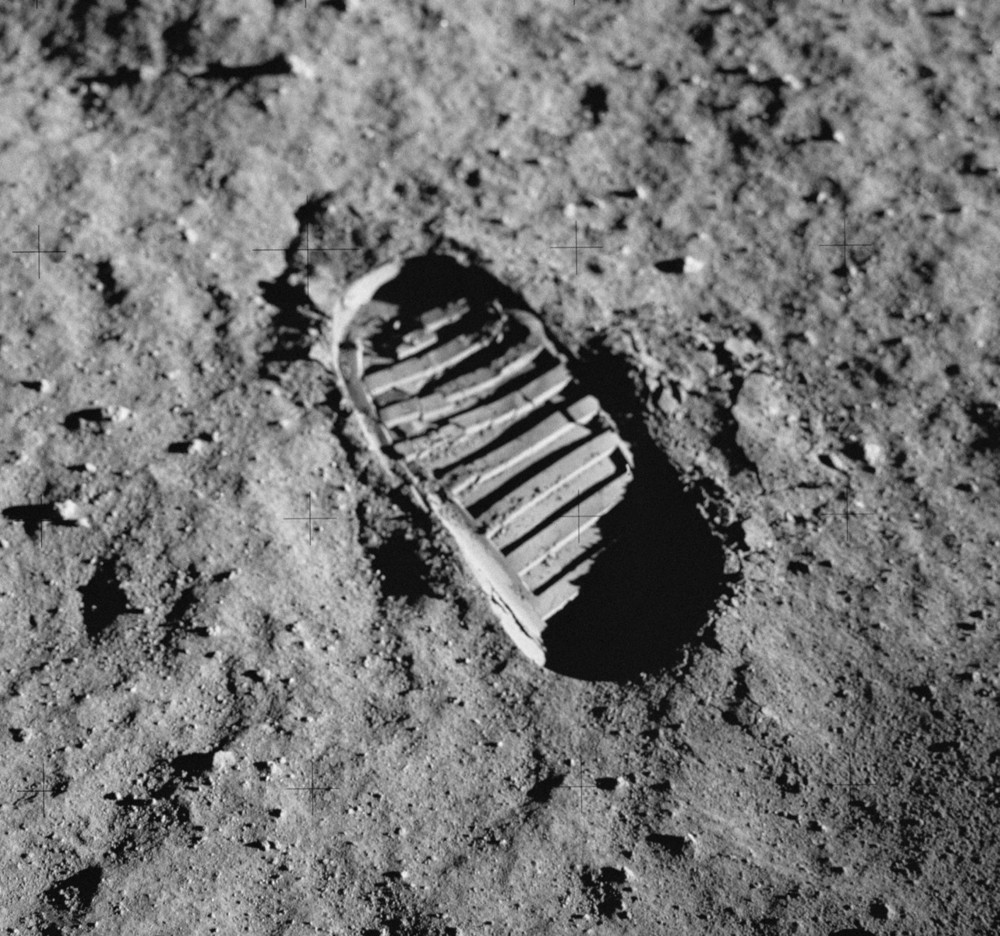
\includegraphics[height=0.4\textheight]{images/apollo-footprint.jpg}
		\end{column}
		\begin{column}{0.6\textwidth}
			Pros:
			\begin{itemize}
				\item Daniel have gotten experience of standard Unity engine utilization for VR tasks and became familiar with pitfalls to avoid
			\end{itemize}
			Cons:
			\begin{itemize}
				\item No source code available!
			\end{itemize}
		\end{column}
	\end{columns}
	\centering
	.\newline\newline
	The first step was done! We start from the scratch now and have more options to adjust the future system to your needs!\\
	%(Daniel will be happy to answer your questions about VR)
\end{frame}

\section{Deep Learning}
\subsection{Subsection1}
\begin{frame}{What is Deep Learning?}
	\begin{columns}
		\begin{column}{0.45\textwidth}
			\begin{figure}
				\centering
				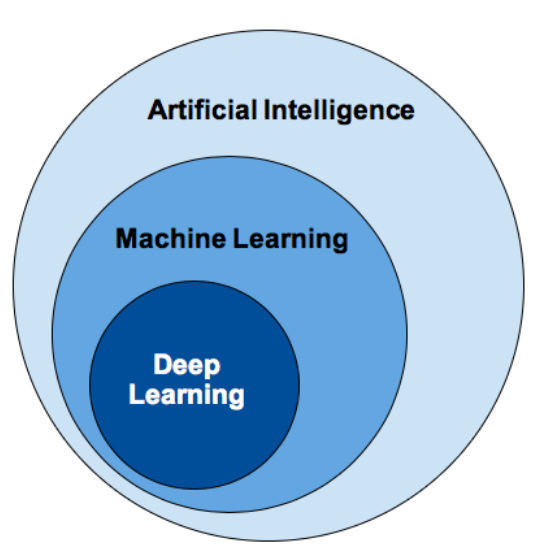
\includegraphics[width=\textwidth]{images/ai_ml_dl.png}
			\end{figure}
		\end{column}
		\begin{column}{0.55\textwidth}
			\begin{itemize}
				\item AI - mimics human behaviour;
				\item ML - use statistical methods to improve machines performance with experience;
				\item DL - use neural networks; \textit{creates features on its own}.
			\end{itemize}
		\end{column}
	\end{columns}
\end{frame}

\subsection{Subsection1}
\begin{frame}{Why Deep Learning if Random Forest works fine for us?}
	\begin{columns}
		\begin{column}{0.45\textwidth}
			\begin{figure}
				\centering
				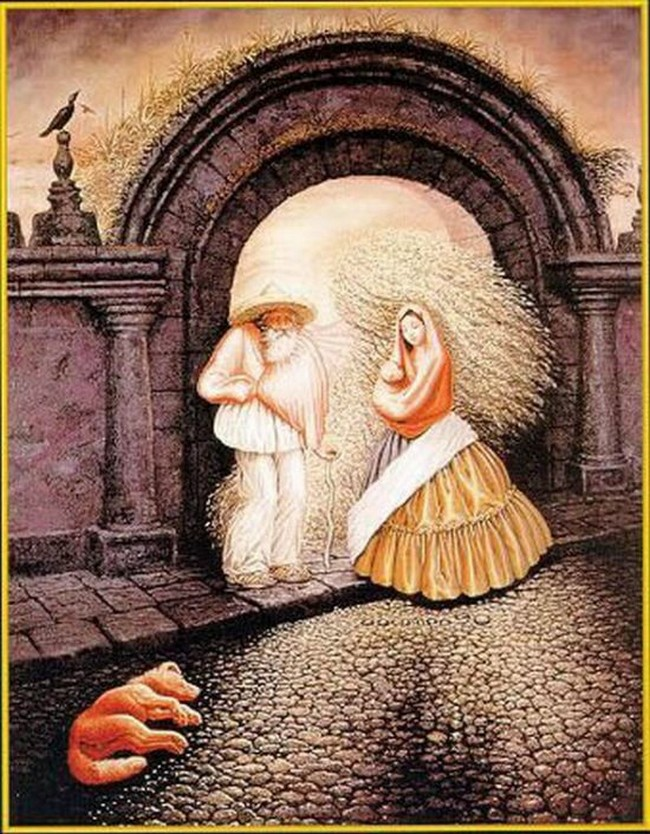
\includegraphics[width=\textwidth]{images/dali.jpg}
			\end{figure}
		\end{column}
		\begin{column}{0.55\textwidth}
			There are different approaches:
			\begin{itemize}
				\item Linear Models (Logistic regression, SVM);
				\item \textbf{Tree Based Methods (i. e. Random Forest);}
				\item \textbf{Deep Learning (Neural Networks);}
				\item kNN.
			\end{itemize}
			All of them has benefits and drawbacks, more suitable for different tasks and data (no free lunch theorem).
		\end{column}
	\end{columns}
\end{frame}

\subsection{Subsection2}
\begin{frame}{Computer vision: images are numbers}
\begin{figure}
	\centering
	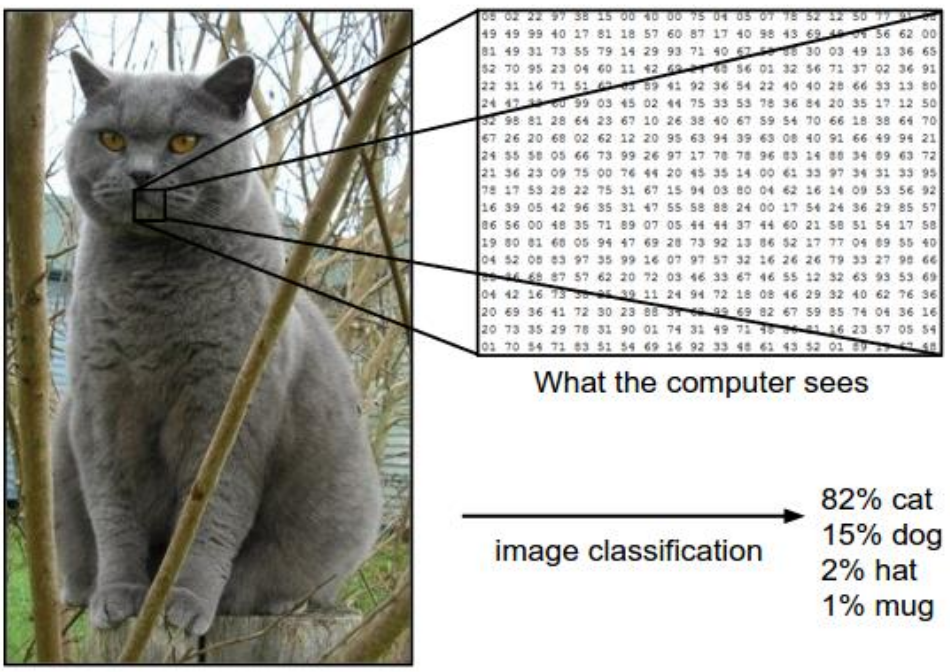
\includegraphics[width=.8\textwidth]{images/cat_array.png}
	\caption{\href{https://deeplearning.mit.edu}{{\color{blue}\underline{MIT 6.S094}}}}
\end{figure}
\end{frame}

\subsection{Subsection3}
\begin{frame}
\frametitle{IJC: Methilation data classifier}
	\begin{columns}
		\begin{column}{0.5\textwidth}
			\textbf{Step 1:}
			\newline
			Convert interrogated cpg for patient:
			\newline
			[0.92, 0.77, 0.81, ..., 0.09, 0.62]
			to the image:
			\begin{figure}
				\centering
				
\includegraphics[height=0.4\textheight]{images/methilation_data.png}
			\end{figure}
		\end{column}
	\begin{column}{0.5\textwidth}
		\textbf{Step 2:}
		\newline
		Build image classifier, results:
		\newline
		\begin{figure}
			\centering
			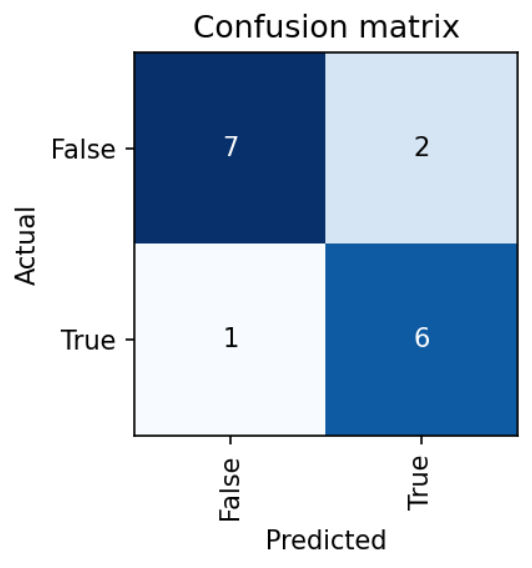
\includegraphics[height=0.55 \textheight]{images/cm_methilation.png}
		\end{figure}
	\end{column}
\end{columns}
\textbf{Resume:} preliminary result provided by neural networks perform as classical ML approaches (and provide higher accuracy than in the \href{http://diposit.ub.edu/dspace/bitstream/2445/125743/1/Esteller\_\%202018.pdf}{{\color{blue}\underline{paper}}}).
\end{frame}

\subsection{Subsection4}
\begin{frame}{MoLAB: MRI segmentation}
	\begin{columns}
		\begin{column}{0.5\textwidth}
			\begin{figure}
				\centering
				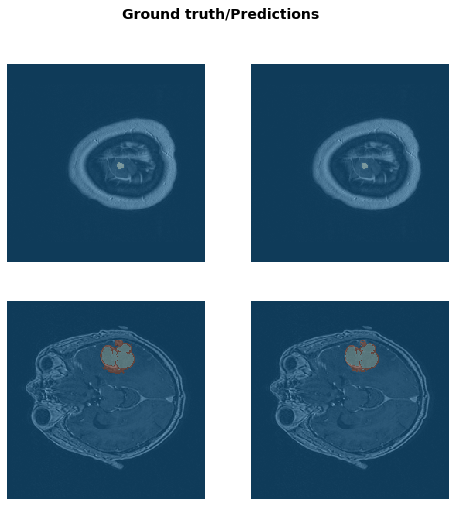
\includegraphics[height=.8\textheight]{images/segmentation.png}
			\end{figure}
		\end{column}
	\begin{column}{0.4\textwidth}
		Data quality and quantity defines quality of results. Labelled data is required.
		\newline
		\begin{center}
			\begin{tabular}{ |c|c| } 
				\hline
				Type & \# of MRIs \\
				\hline
				Meningioma & 276 \\
				\hline
				HGG & 528 \\ 
				\hline
				Metastasis & 264 \\
				\hline
				\textbf{Total} & \textbf{1068} \\
				\hline
			\end{tabular}
		\end{center}
	\end{column}
	\end{columns}
\end{frame}

\subsection{Subsection5}
\begin{frame}{MoLAB: MRI classification \& interpretability}
	\begin{figure}
		\centering
		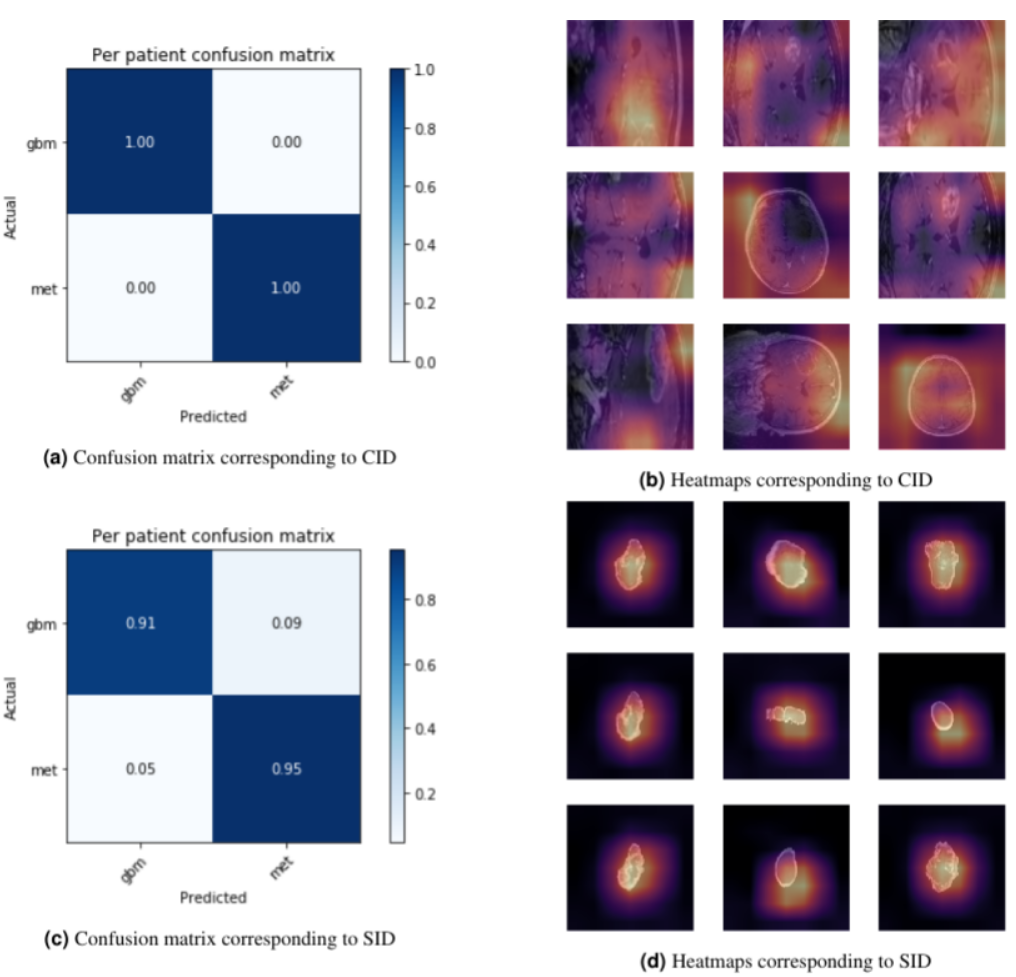
\includegraphics[height=.8\textheight]{images/molab.png}
		\caption{Qualification of DL-engineer is more important than data.}
	\end{figure}
\end{frame}

\subsection{Subsection6}
\begin{frame}\frametitle{Deep Learning applications}
	\begin{columns}
		\begin{column}{0.5\textwidth}
			\begin{figure}
				Deep Learning solved protein folding problem.
				\centering
				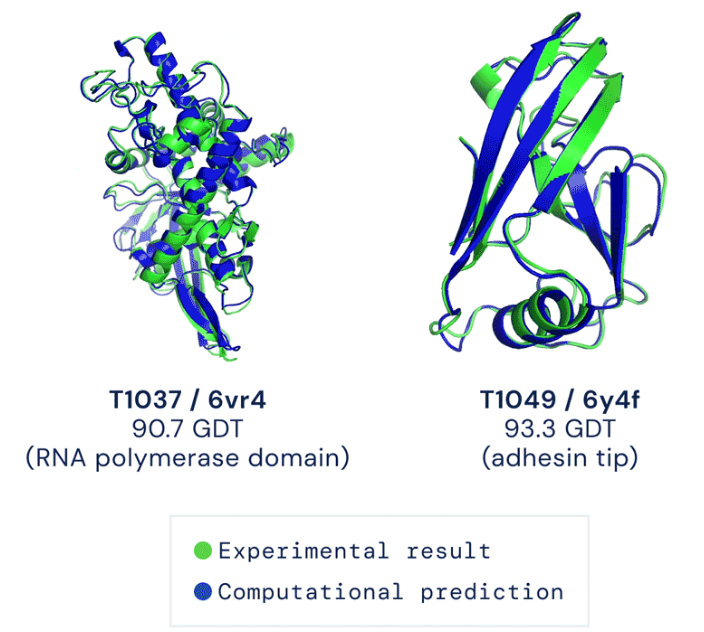
\includegraphics[height=.5\textheight]{images/deep_mind.png}
				\caption{\href{https://deepmind.com/blog/article/alphafold-a-solution-to-a-50-year-old-grand-challenge-in-biology}{{\color{blue}\underline{DeepMind blog post}}}}
			\end{figure}
		\end{column}
		\begin{column}{0.5\textwidth}
			Synthetic MRI generation.
			\begin{figure}
				\centering
				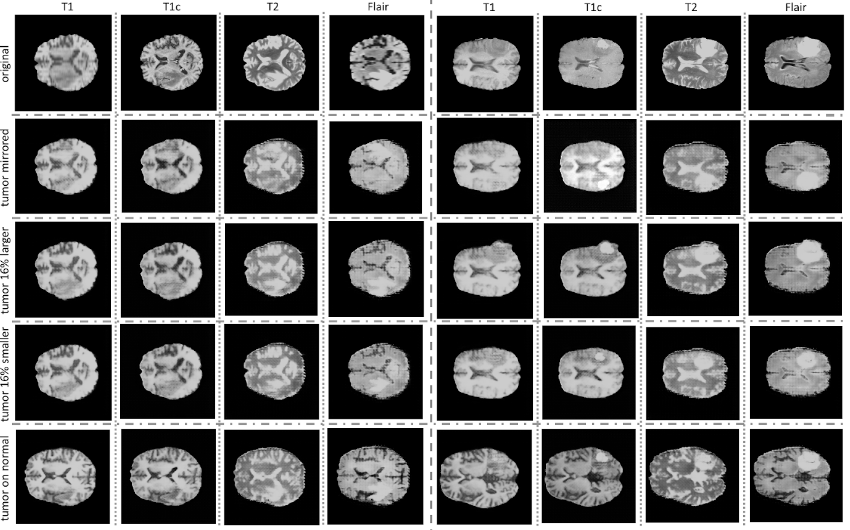
\includegraphics[height=.4\textheight]{images/mri_generation.png}
				\caption{\href{https://news.developer.nvidia.com/ai-can-generate-synthetic-mris-to-advance-medical-research/}{{\color{blue}\underline{NVidia blog post}}}}
			\end{figure}
		\end{column}
	\end{columns}
\end{frame}

\subsection{Subsection7}
\begin{frame}\frametitle{Deep Learning applications}
	\begin{columns}
	\begin{column}{0.5\textwidth}
		\begin{figure}
			\centering
			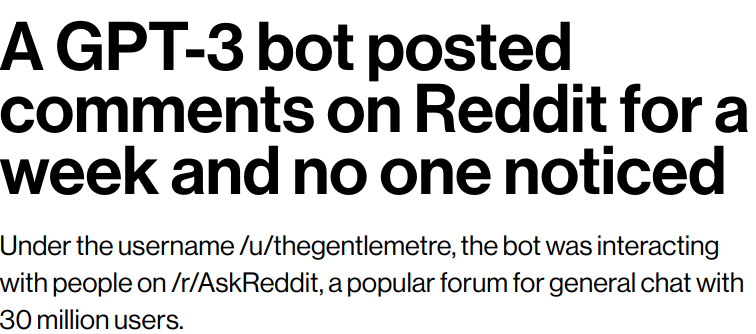
\includegraphics[height=.3\textheight]{images/reddit.png}
			\caption{\href{https://www.technologyreview.com/2020/10/08/1009845/a-gpt-3-bot-posted-comments-on-reddit-for-a-week-and-no-one-noticed/}{{\color{blue}\underline{Blog post}}}}
		\end{figure}
	GPT-3 model: \href{https://arxiv.org/abs/2005.14165}{{\color{blue}\underline{paper}}}
	\end{column}
	\begin{column}{0.5\textwidth}
		Navier–Stokes equations - important hydrodynamics model.
		\begin{figure}
			\centering
			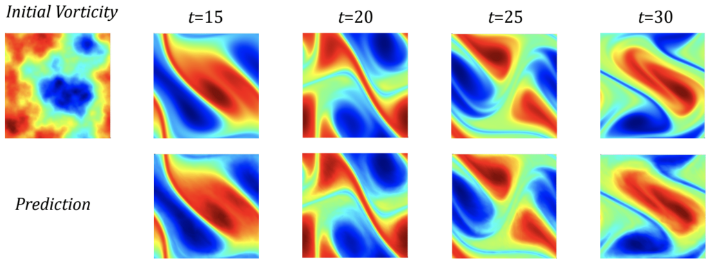
\includegraphics[height=.32\textheight]{images/navie.png}
			\caption{\href{https://arxiv.org/abs/2010.08895}{{\color{blue}\underline{Navier-Stokes equation solver $10^3$ speed-up}}}}
		\end{figure}
	\end{column}
\end{columns}
\end{frame}


\subsection{Subsection9}
\begin{frame}
\frametitle{Conclusions}
\begin{columns}
	\begin{column}{0.6\textwidth}
		\centering
		
\includegraphics[height=0.7\textheight]{images/i-know-ml.png}
	\end{column}
	\begin{column}{0.4\textwidth}
		
		\begin{itemize}
			\item Deep Learning is valuable addition to IJC's tools-set ("AGATA" project?);
			\item Classical ML is still "the thing";
			\item I am happy to share my DL knowledge and expertise
		\end{itemize}
	\end{column}
\end{columns}
\end{frame}

\section{Discussion}
\subsection{Subsection1}
\begin{frame}{Discussion}
	\begin{columns}
		\begin{column}{0.45\textwidth}
			\begin{figure}
				\centering
				
\includegraphics[width=.7\textwidth]{images/qrcode.png}
			\end{figure}
		\end{column}
		\begin{column}{0.55\textwidth}
			\begin{itemize}
				\item Most of AI starups fail not because they have bad ML-models... but because they solve not relevant problems.
				\item What problems in your everyday work may be solved with the help of VR or DL or their combination?
			\end{itemize}
		\end{column}
	\end{columns}
\centering
\textbf{Thank you for your attention!}
\end{frame}

\end{document}